We will measure now the execution time of our solution, that we called \textbf{bwa-gasal2}, and compare it to the mainline version of BWA-MEM version 0.7.17~\cite{lh3:bwa}, the latest release at the time of writing. For the measurements, bwa-gasal2 processes sequences in batches of 1000, which gives between 10 000 and 100 000 seeds to process in a single GPU stream.

\subsection{Data set SRR150}

For the first data set, full program execution times are given in Figure~\ref{fig:total-exec-time-srr150} and kernel speed-ups against BWA-MEM in Figure~\ref{fig:total-exec-speed-up-srr150}. We can notice that the global speed-up fluctuates quite a lot when using different threads, but no trend can be inferred. This may be due to our testing conditions or simply due to the nature of the data set, the results may present uneven behaviour depending on how data is split between threads. As we will see later on, the global speed-up profile with respect to the number of threads has a more consistent trend with the second data set.

\begin{figure}[p]
	\centering
	\begin{subfigure}[t]{1\textwidth}
		\centering
			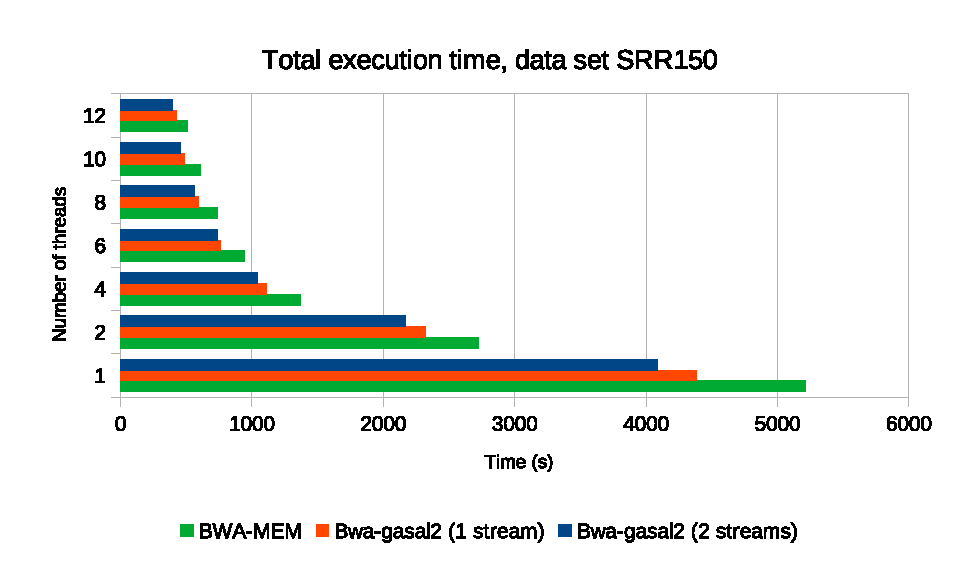
\includegraphics[width=1\textwidth]{srr150/total-exec-time-srr150}
		\caption{Total execution time for SSR150}
		\label{fig:total-exec-time-srr150}
	\end{subfigure}%
	
	\begin{subfigure}[b]{1\textwidth}
		\centering
		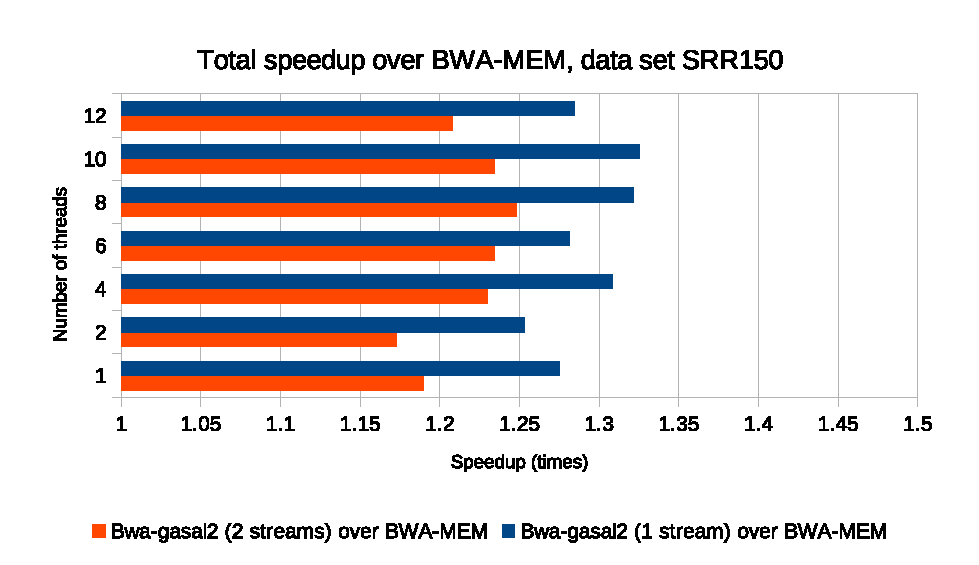
\includegraphics[width=1\textwidth]{srr150/total-exec-speed-up-srr150}
		\caption{Speed-up for the whole program execution for SRR150}
		\label{fig:total-exec-speed-up-srr150}
	\end{subfigure}
	\caption{Program results for data set SRR150}
	%\label{fig:}
\end{figure}

We obtain the most important speed-up using a single thread, reaching 1.35$\times$ the original program speed. This is promising, but is hardly a good indicator: in fact, these kind of program are usually run with multiple threads, and as we mentioned on Chapter~\ref{chap:accel}, a single thread running the accelerator is far from sufficient to saturate the GPU computing resources.

In the case of 12 threads, the total speed-up almost reaches 1.28$\times$. It is below our theoretical maximum of 1.37$\times$, but it is still an important acceleration. Many factors can participate in making this difference. In particular, memory filling for the batches requires a significant amount of time on the CPU side, in addition to the memory copies from host to device. In this case, we started with an already large memory allocation, to avoid any overhead caused by new allocations.

In all cases, the difference between one and two streams is striking, with the speed-up even leaping from 1.21$\times$ to 1.28$\times$ in the 12 threads case.

When isolating the kernel times and kernel speed-up, we get the measurements shown respectively in Figure~\ref{fig:kernel-exec-time-srr150} and Figure~\ref{fig:kernel-exec-speed-up-srr150}. It is important to notice that what is reported as "kernel time" for the 2-stream variant represents only the time during which the CPU is actively waiting for the GPU results. In other words, we have disabled overlapped execution when using one stream, and enabled with 2 streams. We call this "visible kernel execution time".


\begin{figure}[p]
	\centering
	\begin{subfigure}[t]{1\textwidth}
		\centering
		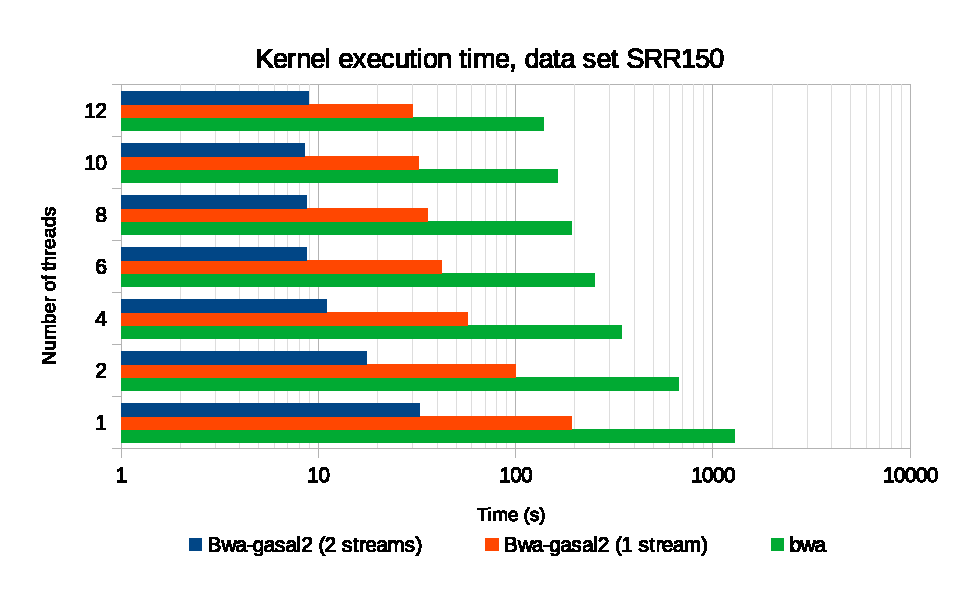
\includegraphics[width=1\textwidth]{srr150/kernel-exec-time-srr150}
		\caption{Visible kernel execution time for SRR150}
		\label{fig:kernel-exec-time-srr150}
	\end{subfigure}%
	
	\begin{subfigure}[b]{1\textwidth}
		\centering
		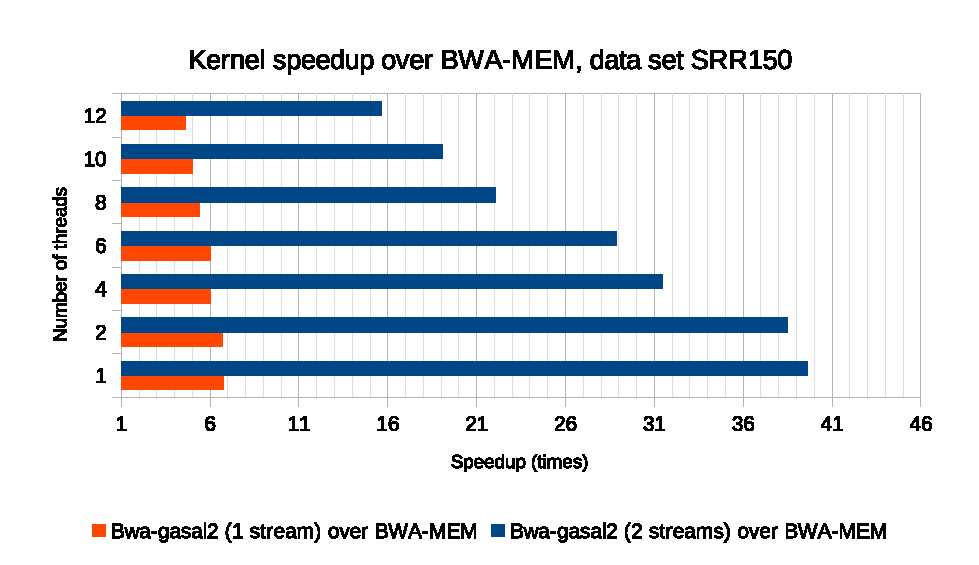
\includegraphics[width=1\textwidth]{srr150/kernel-exec-speed-up-srr150}
		\caption{Speed-up for the kernel execution for SRR150}
		\label{fig:kernel-exec-speed-up-srr150}
	\end{subfigure}
	\caption{Kernel results for data set SRR150}
	%\label{fig:}
\end{figure}

With overlapped execution, in the 2-stream version, the visible kernel time is an order of magnitude shorter. In this case, the kernel times were hugely different, so we had to display them in log scale. While the speed-up reaches 4.7$\times$ in single stream with 12 threads, it jumps to almost 16$\times$, effectively shrinking down the compute time of the extension by the same amount. Single-thread results are even more impressive, with a  kernel speed-up reaching 40$\times$ with overlapping, and only 6$\times$ when actively waiting for the result.


\subsection{Data set SRR250}

We run the same measurements on data set SRR250. Its reads are longer, so they take quite a substantial amount of time to complete. Execution times and overall speed-up are shown in Figure~\ref{fig:total-exec-time-srr250} and Figure~\ref{fig:total-exec-speed-up-srr250}, respectively.


\begin{figure}[p]
	\centering
	\begin{subfigure}[t]{1\textwidth}
		\centering
		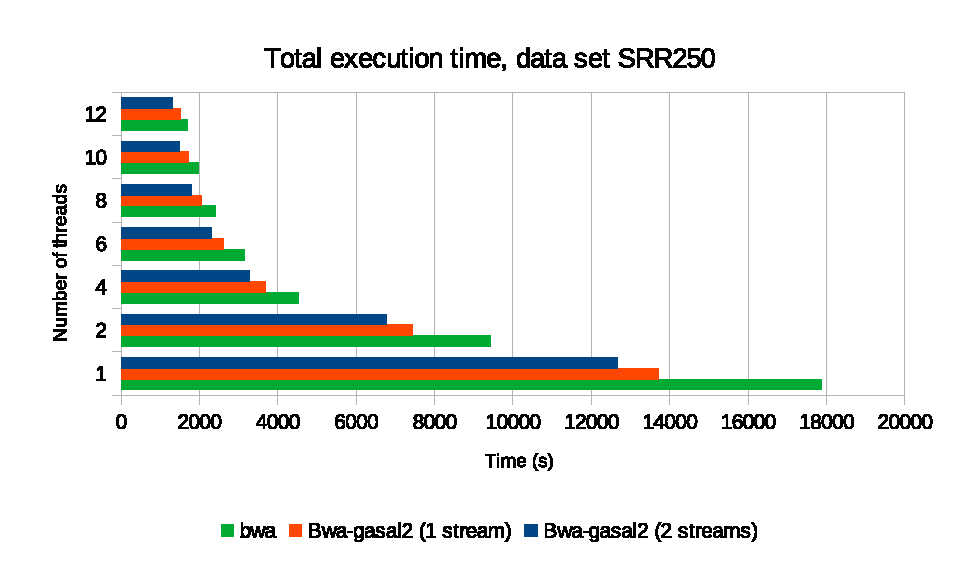
\includegraphics[width=1\textwidth]{srr250/total-exec-time-srr250}
		\caption{Total execution time for SSR250}
		\label{fig:total-exec-time-srr250}
	\end{subfigure}%
	
	\begin{subfigure}[b]{1\textwidth}
		\centering
		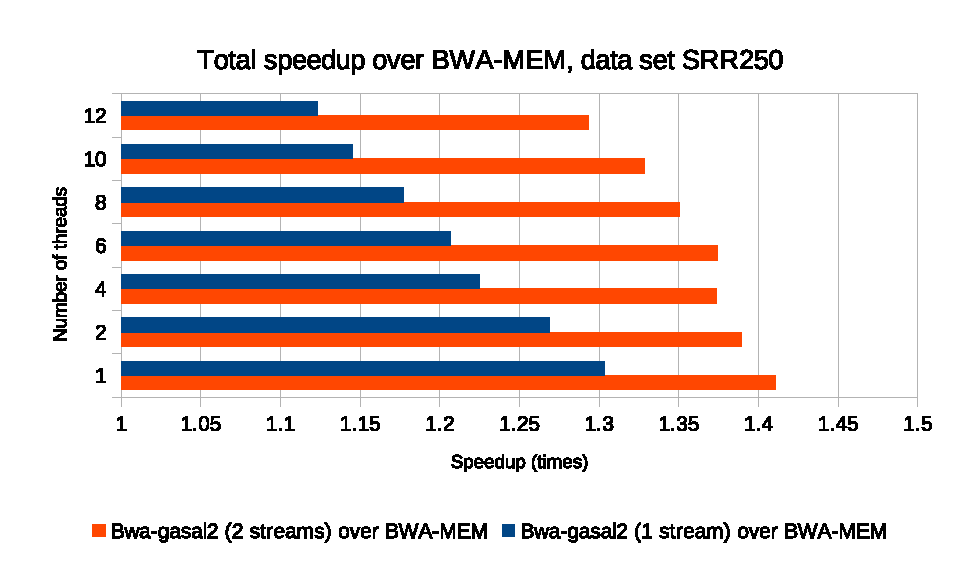
\includegraphics[width=1\textwidth]{srr250/total-exec-speed-up-srr250}
		\caption{Speed-up for the whole program execution for SRR250}
		\label{fig:total-exec-speed-up-srr250}
	\end{subfigure}
	\caption{Program results for data set SRR250}
	%\label{fig:}
\end{figure}

For this data set, the extension time is taking approximately 33\% of the total time, so we would expect a bigger speed-up, with the theoretical maximum being 1.5$\times$. With 2 streams and single thread, we can effectively reach a speed-up of 1.41$\times$, which gets somewhat close to the theoretical maximum. With 12 threads, the speed-up is 1.29$\times$. This is still a valuable improvement over the original version, and in all cases, overlapped execution gives a substantial boost in performance. When comparing the single stream version to its 2-stream counterpart, we note that using 2 streams definitely helps shrinking the execution time.

We will now examine the kernel times and speed-up, in Figure~\ref{fig:kernel-exec-time-srr250} and Figure~\ref{fig:kernel-exec-speed-up-srr250} respectively.


\begin{figure}[p]
	\centering
	\begin{subfigure}[t]{1\textwidth}
		\centering
		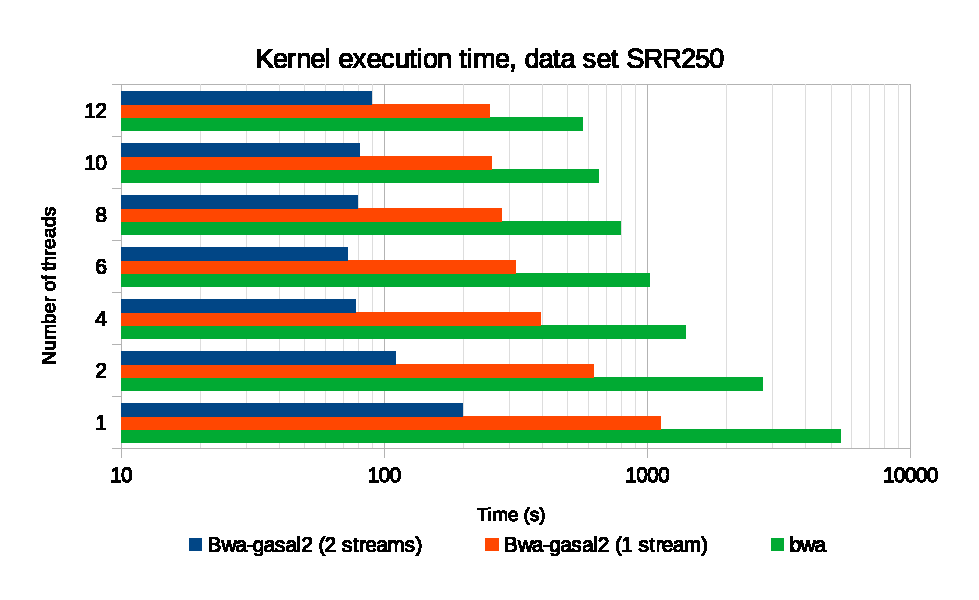
\includegraphics[width=1\textwidth]{srr250/kernel-exec-time-srr250}
		\caption{Visible kernel execution time for SRR250}
		\label{fig:kernel-exec-time-srr250}
	\end{subfigure}%
	
	\begin{subfigure}[b]{1\textwidth}
		\centering
		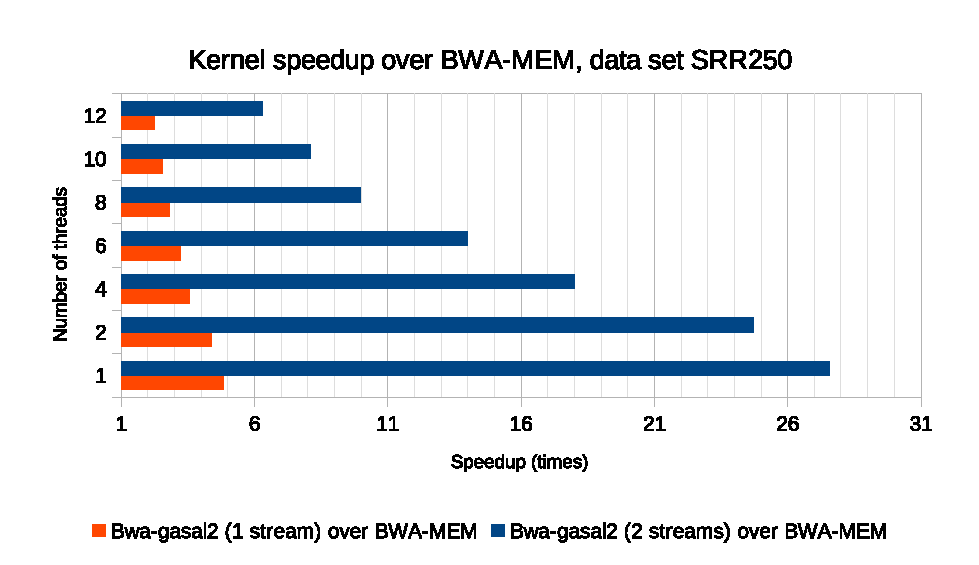
\includegraphics[width=1\textwidth]{srr250/kernel-exec-speed-up-srr250}
		\caption{Speed-up for the kernel execution for SRR250}
		\label{fig:kernel-exec-speed-up-srr250}
	\end{subfigure}
	\caption{Visible kernel execution for data set SRR250}
	%\label{fig:}
\end{figure}

Kernel running times for BWA-MEM (running on CPU) are steady. As the number of threads increases, we get closer to a plateau as the execution time hardly gets any lower for all programs. Again, we can remark how overlapped execution helps in computing it faster with two streams. The difference is tremendously high for one thread, with the CPU waiting time for the GPU to complete being 5 times lower with 2 streams (from 1125s with 1 stream to 197s). When using 12 threads, the time the CPU waits for the kernel to finish is 2.5 lower for the 2-stream version (from 250s for 1 stream to 89s for 2 streams). When using multiple threads, the overhead caused by filling a lot of GPU batches and copying them to the device is substantial. It is all the more the case when using twice as many streams, having twice as many structures needing filling and being copied to the device. This could explain why the speed-up boost got from the overlapped execution tends to get smaller with longer reads for 2 streams.

We can also see whether increasing the number of streams could give any performance improvement. Results are shown in Figure~\ref{fig:exec-time-nbstreams}. As we can see, using more than 2 streams does not provide in any improvement. 

\begin{figure}[h]
	\centering
	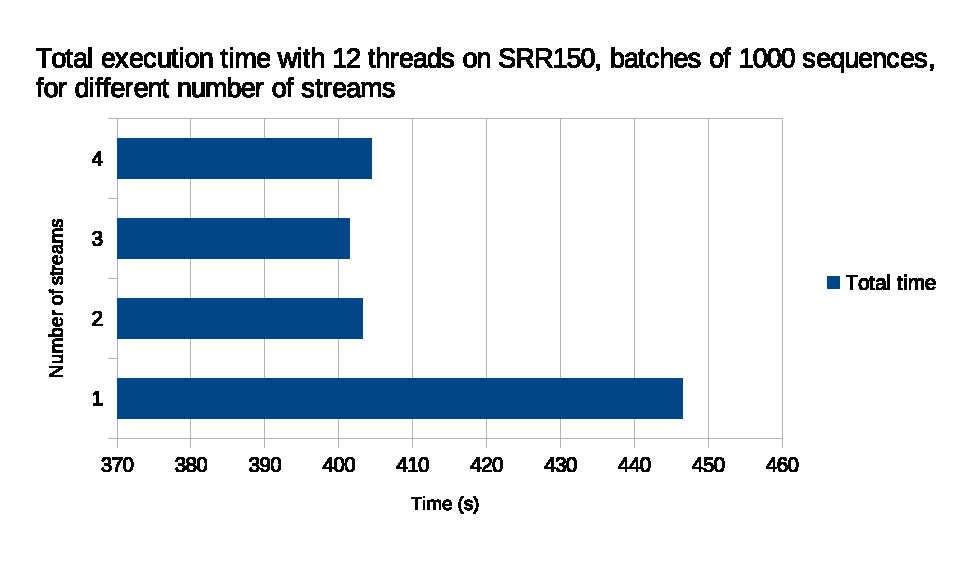
\includegraphics[width=0.9\linewidth]{exec-time-nbstreams}
	\caption{Execution time for 12 threads and different number of streams, data set SRR150}
	\label{fig:exec-time-nbstreams}
\end{figure}

% Note: this newpage is nice here, but depending on the content above, it may be ugly.
% \newpage